\documentclass[paper=a4, fontsize=11pt]{scrartcl} % KOMA-article class

%-------------------------------------------------
%   THEMES, PACKAGES, CUSTOM COMMANDS
%-------------------------------------------------
\usepackage{blindtext}
\usepackage[english]{babel}                             % English language/hyphenation
\usepackage[protrusion=true,expansion=true]{microtype}  % Better typography
\usepackage{amsmath,amsfonts,amsthm,mathtools}                    % Math packages
\usepackage[pdftex]{graphicx}                           % Enable pdflatex
\usepackage[export]{adjustbox}
\usepackage[svgnames]{xcolor}                           % Enabling colors by their 'svgnames'
\usepackage[hang, small,labelfont=bf,up,textfont=it,up]{caption} % Custom captions under/above floats
\usepackage{subcaption}
\usepackage{epstopdf}       % Converts .eps to .pdf
%\usepackage{subfig}         % Subfigures
\usepackage{booktabs}       % Nicer tables
\usepackage{fix-cm}         % Custom fontsizes
\usepackage{listings}
\usepackage{soul}

\usepackage[foot=30pt,margin=1in]{geometry}

% Custom sectioning (sectsty package)
\usepackage{sectsty}
\allsectionsfont{
    \usefont{OT1}{phv}{b}{n}    % bch-b-n: CharterBT-Bold font
}
\sectionfont{
    \usefont{OT1}{phv}{b}{n}
}

% Custom colors
\definecolor{brsugrey}{rgb}{0.9, 0.9, 0.9}
\definecolor{brsublue}{rgb}{0, 0.594, 0.949}

%
\newcommand{\upperRomannumeral}[1]{\uppercase\expandafter{\romannumeral#1}}

% Creating an initial of the very first character of the content
\usepackage{lettrine}
\newcommand{\initial}[1]{%
    \lettrine[lines=3,lhang=0.3,nindent=0em]{
        \color{brsublue}
        {\textsf{#1}}}{}}

%-------------------------------------------------
%   COMMON INFO
%-------------------------------------------------
\newcommand{\hmwkTitle}{Homework 2}
\newcommand{\hmwkDueDate}{Lecture date: 10 October 2016}
\newcommand{\hmwkClass}{Neural Networks}
\newcommand{\hmwkClassShort}{NN WS2016}
\newcommand{\hmwkAuthorFullName}{Minh H. Nguyen}
\newcommand{\hmwkAuthorLastName}{Nguyen}
\newcommand{\hmwkAuthorEmail}{minh.nguyen@smail.inf.h-brs.de}
\newcommand{\hmwkAuthorInstitute}{BRS University of Applied Sciences}

%-------------------------------------------------
%   HEADERS & FOOTERS
%-------------------------------------------------
\usepackage{fancyhdr}
\pagestyle{fancy}
\usepackage{lastpage}
% Header (empty)
\lhead{}
\chead{}
\rhead{}
% Footer (you may change this to your own needs)
\lfoot{\footnotesize
    \texttt{\hmwkClassShort} ~
    \textbullet ~ \hmwkAuthorLastName ~
    \textbullet ~ \hmwkTitle}
\cfoot{}
\rfoot{\footnotesize page \thepage\ of \pageref{LastPage}}  % "Page 1 of 2"
\renewcommand{\headrulewidth}{0.0pt}
\renewcommand{\footrulewidth}{0.4pt}

%-------------------------------------------------
%   TITLE & AUTHOR
%-------------------------------------------------
\usepackage{titling}

\newcommand{\HorRule}{\color{brsublue}% Creating a horizontal rule
    \rule{\linewidth}{1pt}%
    \color{black}
}

% Title
\pretitle{
    \begin{flushleft}
        \HorRule
        \fontsize{25}{25} \usefont{OT1}{phv}{b}{n} \color{gray} \selectfont
}
\title{\hmwkClass \\
       \hmwkTitle}
\posttitle{
    \par
    \end{flushleft}
}

% Author
\preauthor{
    \begin{flushleft}
        \large \lineskip 0.25em
        \usefont{OT1}{phv}{b}{sl} \color{brsublue}}

\author{\hmwkAuthorFullName}

\postauthor{
        \footnotesize
        \usefont{OT1}{phv}{m}{sl} \color{Black}
        \\\hmwkAuthorInstitute
        \\\hmwkAuthorEmail
        \par
    \end{flushleft}
    \HorRule}

% Date
\date{\hmwkDueDate}

%-------------------------------------------------
%   BEGIN
%-------------------------------------------------
\begin{document}
    \maketitle
    \thispagestyle{fancy} % Enabling the custom headers/footers for the first page

    \section*{Text Summary}

    Title: \textit{Neural Networks: A Comprehensive Foundation} by Haykin Simons, chapter 2 - Learning Processes.

    \begin{itemize}
        \item Learning process definition:
        \begin{itemize}
            \item Sequence of events that take place:
            \begin{enumerate}
                \item Neural network is stimulated by an environment
                \item Simulation causes changes in the network's free parameter
                \item Network responds to the environment differently because of these changes
            \end{enumerate}
            \item Type of learning is determined by how the parameters are changed.
        \end{itemize}

        \item Types of learning:
        \begin{itemize}
            \item Error-correction learning
            \begin{center}
                %\setlength{\fboxsep}{0.5pt} %
                %\setlength{\fboxrule}{0.5pt} %,fbox
                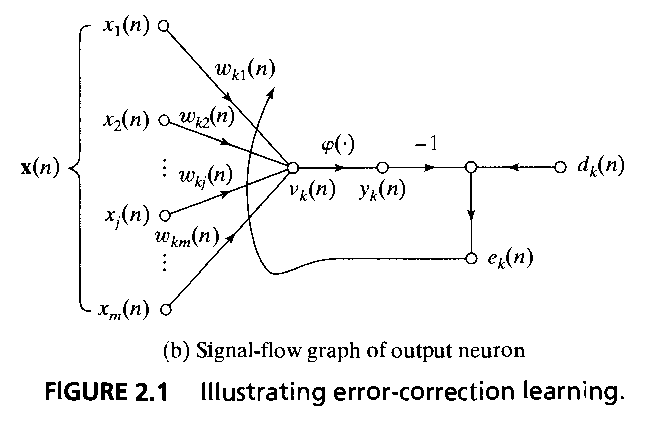
\includegraphics[width=14.0cm]{../images/Haykin-NN-figure2-1.png} %
            \end{center}

            Update rule for synaptic weight for neuron $k$:
                \[ w_{kj}(n+1) = w_{kj}(n) + \Delta w_{kj}(n) \]
                where adjustment $\Delta w_{kj}(n)$ for excitement $x_j(n)$ and error signal $e_k(n)$ is:
                \[ \Delta w_{kj}(n) = \eta e_k(n)x_j(n) \]

            \item Memory-based learning: updates for new test vector use old data from the ``local neighborhood'' of the new data point. Learning involves:
            \begin{itemize}
                \item criterion for defining the neighborhood
                \item learning rule applied to this neighborhood
            \end{itemize}
            KNN learning:
            \begin{itemize}
                \item Identify $k$ classified patterns nearest to test vector.
                \item Assign test vector to class most frequently represented in the $k$ neighbors.
            \end{itemize}

            \item Hebbian learning - two rules:
            \begin{itemize}
                \item strength of synapse increases if the two neurons on either side are activated simultaneously (synchronously).
                \item strength decreases if the two neurons are activated asynchronously.
            \end{itemize}
            Four key properties:
            \begin{itemize}
                \item time-dependent: modification to synapse depends on time of occurrence of presynaptic and postsynaptic signals.
                \item local mechanism: information bearing signals are in ``spatiotemporal contiguity.''
                \item interactive mechanism: change in synapse depends on both sides of the synapse
                \item conjunctional or correlational mechanism.
            \end{itemize}

            \item Competitive learning: only one output neuron is active at any one time. Three basic elements:
            \begin{itemize}
                \item set of neurons that respond differently to a given set of inputs.
                \item a limit imposed on the strength of each neuron.
                \item a mechanism for neurons to compete for the right to respond to a subset of inputs.
            \end{itemize}

            \item Boltzmann learning: stochastic learning mechanism based on statistical mechanics.
            \begin{itemize}
                \item  Characterized by an \textit{energy function}:
                \[ E = -\frac{1}{2} \sum_{j} \sum_{k} w_{kj} x_k x_j \]
                where $x_j$ is the state of neuron $j$, weight $w_{kj}$ connects neuron $j$ to $k$, and $j \neq k$.
                \item Each neuron is either in ``on'' ($+1$) or ``off'' ($-1$) state. At some step of learning and some temperature $T$, the state is switched with probability:
                \[ P(x_k \rightarrow -x_k) = \cfrac{1}{1 + \exp(-\Delta E_k/T)} \]
            \end{itemize}
        \end{itemize}

        \item Learning paradigms
        \begin{itemize}
            \item Learning with a teacher - supervised learning:
            \begin{center}
                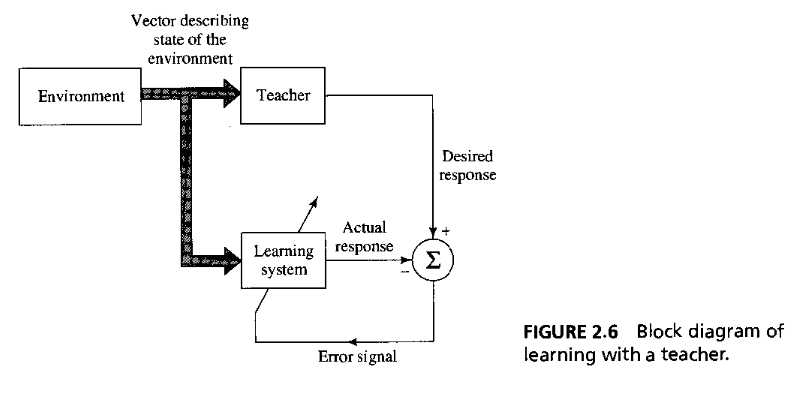
\includegraphics[width=12.0cm]{../images/Haykin-NN-figure2-6.png} %
            \end{center}

            \item Learning without a teacher:
            \begin{itemize}
                \item Reinforcement learning:
                \begin{center}
                    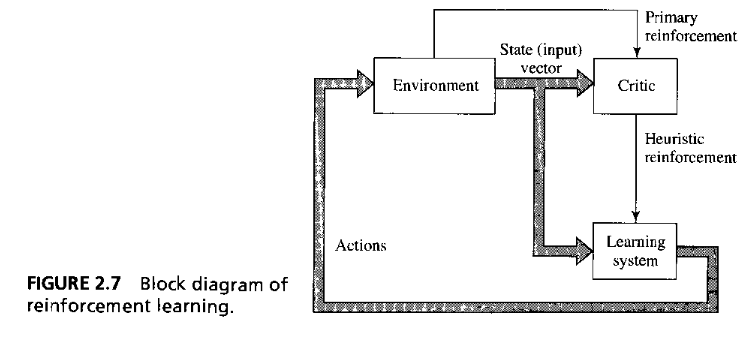
\includegraphics[width=12.0cm]{../images/Haykin-NN-figure2-7.png} %
                \end{center}
                \item Unsupervised learning:
                \begin{center}
                    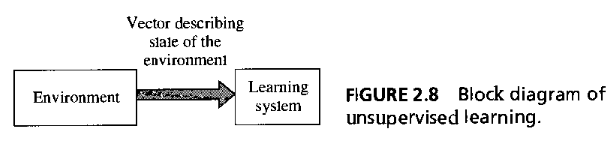
\includegraphics[width=10.0cm]{../images/Haykin-NN-figure2-8.png} %
                \end{center}
            \end{itemize}
        \end{itemize}

    \end{itemize}

    \section*{Exercises}
    \subsection*{Problem 1-13}
    Python code is included in attached notebook. Input-output mapping calculated:
    \tiny
    \[\cfrac{1}{\exp\left(\cfrac{2}{\exp\left(\cfrac{1}{\exp(-2x_1 + 3x_2) + 1} - \cfrac{3}{\exp(-5x_1 - x_2) + 1}\right) + 1} - \cfrac{1}{\exp\left(\cfrac{-6}{\exp(-2x_1 + 3x_2) + 1} - \cfrac{4}{\exp(-5x_1 - x_2) + 1}\right) + 1}\right) + 1}\]
    \normalsize

    \newpage
    Plotting of the classifier:
    \begin{figure}[h!]
        \centering
        \begin{subfigure}[b]{0.65\textwidth}
            \setlength{\fboxsep}{0.5pt} %
            \setlength{\fboxrule}{0.5pt}
            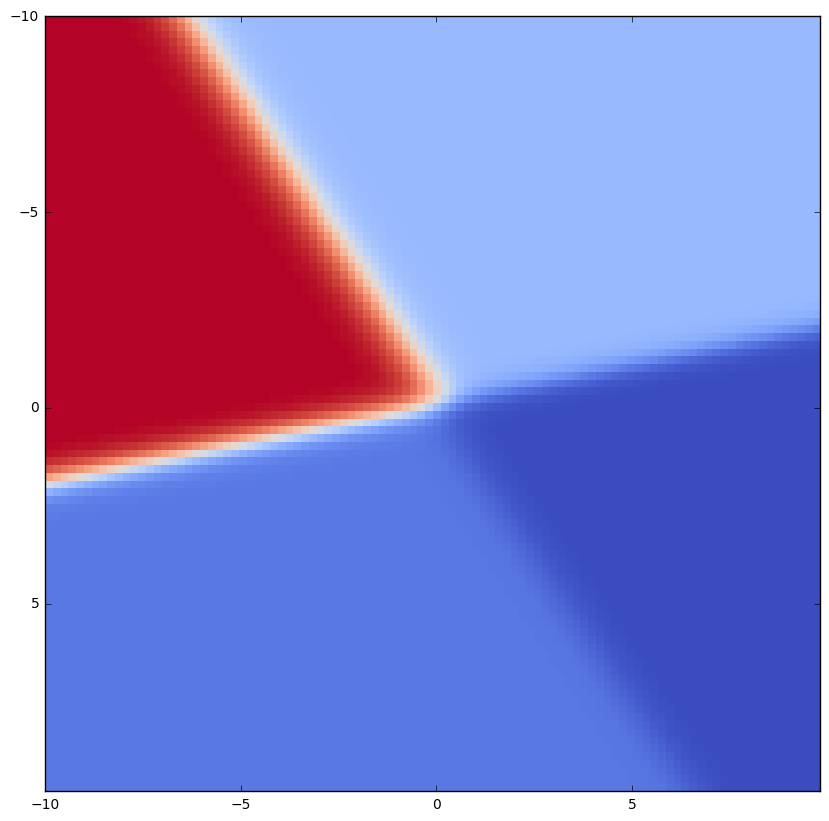
\includegraphics[width=\textwidth,fbox]{../images/NN_MinhNguyen_20161010_ex1-13.png}
            \caption{2D representation}
        \end{subfigure}
        ~
        \begin{subfigure}[b]{0.65\textwidth}
            \setlength{\fboxsep}{0.5pt} %
            \setlength{\fboxrule}{0.5pt}
            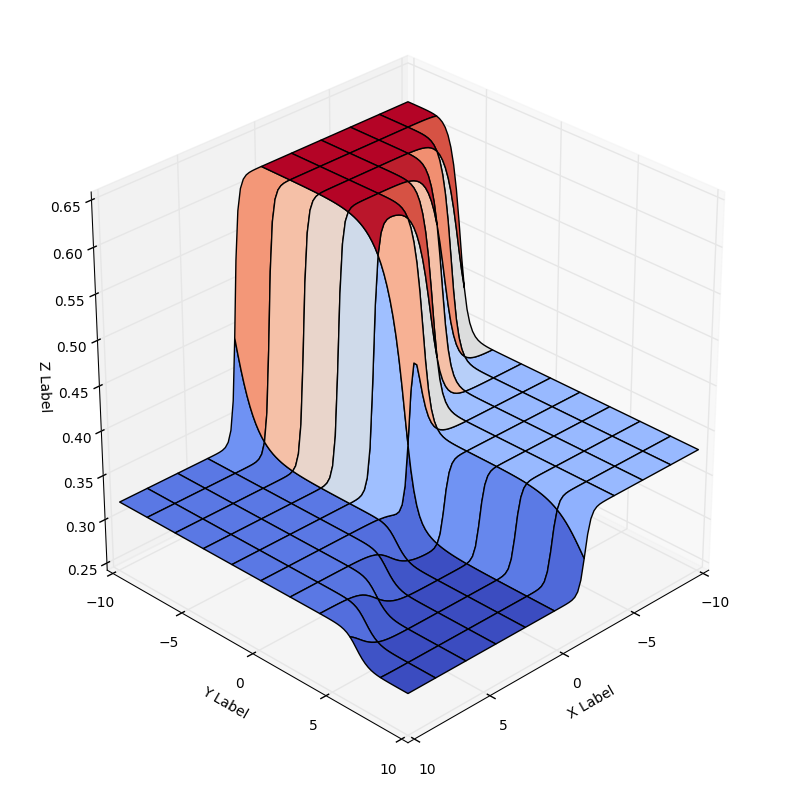
\includegraphics[width=\textwidth,fbox]{../images/NN_MinhNguyen_20161010_ex1-13_3d.png}
            \caption{3D representation}
        \end{subfigure}
        \caption{Illustration of the classification regions of the given network}
    \end{figure}

    \subsection*{Problem in PDF file}
    Calculations are done in the attached Python notebook.

    \subsection*{New classification example with bias}
    Plot of adjusted points:
    \begin{center}
        %\setlength{\fboxsep}{0.5pt} %
        %\setlength{\fboxrule}{0.5pt} %,fbox
        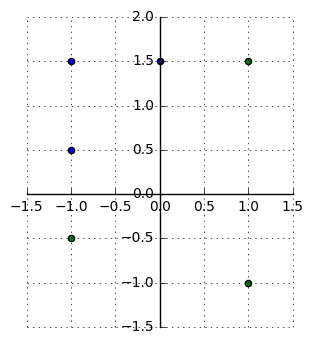
\includegraphics[width=10.0cm]{../images/NN_MinhNguyen_20161010_ex5.png} %
    \end{center}

\end{document}
